% Written report -- Graph Analytics 2026, Albert School.
% Built on the official template (written-report-template.tex): same class,
% packages, section headings and bibliography style. Added only graphicx,
% booktabs and amsmath for figures, tables and the PMI formula.
%
% Skeleton only. Each section and subsection lives in its own file in sections/,
% with one owner per file, so the two branches never edit the same file.
% The %% comments in each file say who writes it, the page
% budget (target 13-14 pages, hard limit 15) and what it must contain, taken
% from the roadmap (https://claude.ai/artifact/6EdHNyEmH9VhYdEhCWCNQa).
% Delete each \guidance{...} line and the %% comments once the section is written.
%
% Owners: A = Khadidja ADDI, B = Mathew Kristoffer Ewan KAPOOR.
% Build: pdflatex main && bibtex main && pdflatex main && pdflatex main
%        (or upload this folder and ../outputs/*.png to Overleaf).

\documentclass[10pt,a4paper]{article}
\usepackage{sectsty}
\usepackage{hyperref}
\usepackage{graphicx}
\usepackage{booktabs}
\usepackage{amsmath}
\sectionfont{\raggedright}
\graphicspath{{../outputs/}}

\newcommand{\guidance}[1]{\par\smallskip\noindent\textit{#1}\par\smallskip}

\title{Communities and Brokers in Ingredient Networks of World Cuisines}
\author{
  Khadidja ADDI\\
  \texttt{kaddi@albertschool.com}%
  \and
  Mathew Kristoffer Ewan KAPOOR\\
  \texttt{mkapoor@albertschool.com}
}
\date{}

\begin{document}
\maketitle

\begin{abstract}
% Owner: B
We ask which communities and connecting nodes emerge from graphs built
on the ingredients of sampled recipes and countries. We project the CulinaryDB
recipe--ingredient bipartite graph~\cite{culinarydb} onto ingredients and
weight retained edges by pointwise mutual information (PMI). We also
build a country graph from a dataset of national dishes~\cite{wunderlich2022data},
using Jaccard similarity between ingredient sets as edge weights. We use
graph statistics, degree, strength, betweenness, Louvain communities and
modularity. We examine articulation points and bridges, compare rankings
with Spearman correlation, and add a shuffle test for agreement with UN
regions. We examine how thresholds change connectivity and modularity.
The ingredient graph has five communities (five in 28 of 30 Louvain
seeds) and modularity $0.400$. Hop betweenness follows frequency ($\rho=0.968$), with Water,
Salt and Butter leading. With $1/\mathrm{PMI}$ distances, Couscous,
Lasagna and Shallot lead, and the correlation is $\rho=0.323$; a second
conversion preserves several leaders but changes their order. Country
communities agree with UN regions for $64.3\%$ of countries, against a
mean of $34.0\%$ over $1{,}000$ shuffles ($p\approx0.001$). We find that
the distance choice changes ingredient broker rankings, while country
communities show a partial association with geography.

\end{abstract}

% ============================================================================
\section{Introduction}
% Owner: B
%% Owner: B. A checks the question matches what was analysed. Budget: 1 page.
\guidance{Introduce the topic and motivation, state the objective, and explain its relevance.}

%% - Motivation: ingredient combinations as relations, which counts cannot show.
%% - Central question (agreed): "What communities and connecting nodes emerge
%%   from ingredient-based graphs of sampled recipes and countries?"
%%   * ingredients: how structural rankings differ from frequency, and how much
%%     they depend on the weighting;
%%   * countries: how communities relate, descriptively, to UN regions.
%% - Prior work: \cite{caprioli2025} studies ingredient-combination networks on
%%   the same CulinaryDB data. Say how this project differs (single ingredients
%%   as nodes, brokers, a second country-level graph) and that their code was
%%   not used.
%% - Methods follow the course \cite{quercini2026}.


% ============================================================================
\section{Dataset Presentation}
% Owner: A
%% Owner: A. B checks every count against the raw files. Budget: 2.5 pages.
\guidance{Describe the dataset and its source, explain how it is represented as a graph, and report relevant graph statistics, including the numbers of nodes and edges.}


\subsection{Sources}\label{sec:sources}
% Owner: A
%% - CulinaryDB \cite{culinarydb}: 45,772 recipes, 26 cuisine labels; PMI uses the
%%   45,749 recipes that have mapped ingredients. Duplicate recipe-ingredient pairs
%%   removed (456,279 -> 412,560). 103 compound ingredients, 95 used, 54 in graph.
%%   Imbalance: USA 16,118 and Italy 7,504 recipes.
%% - EnviDat \cite{wunderlich2022data}: 350 valid dishes (171 national + 179
%%   others), 218 ingredient columns, 171 country/territory labels. cp1252, ';'
%%   separator; one malformed row and one stray value (58) discarded.
%% - UN M49 regions \cite{unregions}, joined on ISO3 (ZAR -> COD, ROM -> ROU).
%% - Why CulinaryDB: downloadable CSV bundle, open licence. Do not say RecipeDB
%%   has no bulk download.
%% - Data are in the GitHub repository with their licences.


\subsection{Ingredient graph}
% Owner: A
We start from the bipartite graph that links each recipe to its ingredients
and project it onto the ingredients, as in the course~\cite{quercini2026}. In
the course projection, two ingredients are linked with a weight equal to
their number of common neighbours, here the number of recipes that contain
both. We change this projection in three ways. We keep only the ingredients
that occur in at least 50 recipes (362 of 695). We keep only the pairs that
share at least 10 recipes. We replace the number of shared recipes by the PMI
of the pair~\cite{church1990} and drop the pairs with PMI $\leq 0$. The result
has 362 nodes and 10{,}853 edges. It is a filtered, PMI-weighted variant of
the taught projection, not the taught projection itself, and PMI is an
extension that the course does not cover. The PMI of two ingredients $i$ and
$j$ is
\begin{equation*}
  \mathrm{PMI}(i,j) = \log_2 \frac{c_{ij}\, N}{c_i\, c_j},
\end{equation*}
where $c_{ij}$ is the number of recipes that contain both ingredients, $c_i$
and $c_j$ are the numbers of recipes that contain each of them, and
$N=45{,}749$ is the number of recipes with at least one ingredient. The
ratio compares how often the pair occurs with how often it would occur if the
two ingredients were independent. A positive PMI means that the pair is more
common than that; it is not a significance test. PMI tends to favour rare
pairs, and the threshold of 10 shared recipes limits this effect.

Shared-recipe counts tell us which pairs are common. PMI tells us which pairs
are more common than their frequencies predict. Table~\ref{tab:pmi} gives two
examples. Salt and garlic occur together in 7{,}571 recipes, but both are so
frequent that about 6{,}554 shared recipes are expected by chance, a ratio of
1.16 (PMI $0.21$). Ginger and soy sauce share fewer recipes (1{,}010) but
about 4.5 times more than expected (PMI $2.16$). On the same 10{,}853 edges,
Louvain finds 3 communities when the weights are the shared-recipe counts and
5 when they are the PMI values. We do not compare the modularity of the two
partitions, because the two weightings define different weighted graphs. We
report this comparison only to show that the weighting changes the groups.

\begin{table}[h]
\centering
\small
\begin{tabular}{@{}l r r r r r@{}}
\toprule
Pair & $c_i$ & $c_j$ & Together & Expected if independent & Ratio \\
\midrule
Salt -- Garlic & 18{,}745 & 15{,}995 & 7{,}571 & 6{,}554 & 1.16 \\
Ginger -- Soybean Sauce & 3{,}418 & 3{,}029 & 1{,}010 & 226 & 4.46 \\
\bottomrule
\end{tabular}
\caption{Recipes that contain both ingredients of a pair, compared with the
number expected if the two ingredients were independent, $c_i c_j / N$. The
ratio is the observed number divided by the expected number; its base-2
logarithm is the PMI. Two examples do not show that PMI is better for every
pair.}
\label{tab:pmi}
\end{table}


\subsection{Country graph}
% Owner: A
%% - Nodes: 171 country/territory labels. Profile: union of ingredients over all
%%   of a country's dishes (national dish only tested as an alternative).
%% - Edges: Jaccard similarity >= 0.30 (Jaccard is used in the course Neo4j lab).
%% - Undirected, simple, weighted. Median profile 16 ingredients; 20 countries
%%   have 8 or fewer, which makes similarities coarse.


\subsection{Graph statistics}
% Owner: B
%% Values re-checked on 8 Nov 2026 against brokers_components.csv,
%% brokers_cut_points.csv, sensibilite_ingredients.csv (10/0.0), and
%% sensibilite_pays.csv (all/0.3) on origin/analysis/brokers-geography.
Table~\ref{tab:stats} summarises both graphs. Both are undirected, simple and
weighted. The ingredient graph is connected, so its diameter and radius cover
all $362$ ingredients. The country graph has five connected components, so we
compute its diameter and radius on the largest one, which holds $166$ of the
$171$ countries (Section~\ref{sec:connectivity}).

\begin{table}[h]
\centering
\begin{tabular}{lrr}
\toprule
Measure & Ingredients & Countries \\
\midrule
Nodes & 362 & 171 \\
Edges & 10{,}853 & 2{,}066 \\
Density & 0.166 & 0.142 \\
Connected components & 1 & 5 \\
Largest component (nodes) & 362 & 166 \\
Diameter / radius of largest component (hops) & 3 / 2 & 6 / 3 \\
Average clustering coefficient & 0.591 & 0.478 \\
Articulation points / bridges & 0 / 0 & 5 / 5 \\
\bottomrule
\end{tabular}
\caption{Required statistics for both graphs. Components outside the country
graph's largest component: Zambia--Zimbabwe, and Grenada, Jordan and Marshall
Islands as isolated nodes.}
\label{tab:stats}
\end{table}


% ============================================================================
\section{Description of the Analysis}
% Owner: A+B
We analyse both graphs with the measures that the course teaches. We first
find the connected components and compute distances and the standard
statistics. We then compare centralities and find communities, and finally we
vary the thresholds that define the graphs. The subsections below give the
software, then the definitions and parameters of each step. The results appear
in the next section.


\subsection{Software}
% Owner: A
We use Python 3.12 with NetworkX 3.7~\cite{hagberg2008}, pandas 3.0.2,
NumPy 2.4.4, SciPy 1.17.1 and Matplotlib 3.10.0. The environment is locked
with \texttt{uv} (file \texttt{uv.lock}), so that the same versions are
installed on every machine. All code, data and results are in the project's
GitHub repository, \url{https://github.com/KHAD5ADDI/Graph-Analytics}. To
reproduce them, run \texttt{uv sync}, then run each script of the
\texttt{src} folder with \texttt{uv run python}, in the order given in the
\texttt{README}. The tables and figures of this report come from one run of
this pipeline on the final version of the repository.


\subsection{Connectivity and distances}\label{sec:connectivity}
% Owner: B
We identify the connected components of each graph. A connected component is
a maximal set of nodes in which a path joins every pair of nodes. We measure
distance as the number of edges, or hops, in a shortest path. Following the
course convention, distance is infinite between nodes in different
components \cite{quercini2026}.

We therefore compute diameter and radius only on the largest connected
component, ignoring edge weights. The diameter is the greatest distance
between any pair of nodes in that component. To obtain the radius, we find
each node's greatest distance to another node, then take the smallest of
these values. These measures describe distances within this component only.

An articulation point (cut vertex) is a node whose removal, together with its
incident edges, increases the number of connected components. A bridge (cut
edge) is an edge whose removal increases that number. We find both with
NetworkX \cite{hagberg2008}.


\subsection{Centrality}
% Owner: B
We use the course definitions of centrality \cite{quercini2026}. Degree counts
neighbours; strength sums incident edge weights. We compute both and hop
betweenness on each graph. We use PMI weights for ingredients and Jaccard
weights for countries.

Betweenness sums, over pairs of other nodes, the share of their shortest
paths that pass through the node considered. Our primary measure of brokers,
meaning ingredients that lie on many shortest paths, is hop betweenness.
We give every edge the same length. NetworkX normalises by the number of
pairs of other nodes: the value is the average share of their shortest paths
passing through the node. Country betweenness uses the whole graph; pairs
in different components contribute nothing.

For sensitivity, we compute betweenness with edge distance $1/\mathrm{PMI}$
and a second conversion, $d=1/(1+\mathrm{PMI})$. Any positive decreasing
function of PMI can define edge lengths, making stronger associations shorter.
The course gives no rule for choosing one. Here PMI ranges from $0.000636$
to $6.643$, so $1/\mathrm{PMI}$ gives extreme distances up to about $1{,}573$.
The second conversion gives distances of $0.131$--$0.9994$. It is still one
choice among many: agreement tests robustness to these two conversions only.
Hop betweenness remains our primary measure.

We also subtract each ingredient's hop-betweenness rank from its degree rank.
A positive rank gap means it ranks higher in betweenness than in degree.
We compare these two taught measures to find betweenness beyond degree,
restricting discussion to the hop top $50$ to avoid gaps among near-zero values.

To compare degree and the betweenness measures with ingredient frequency,
the number of recipes containing the ingredient, we use Spearman
correlation, which compares ranks. We read these correlations descriptively
because frequency comes from the same recipes as the graph. They do not
establish a causal relationship.


\subsection{Communities}
% Owner: A
%% Owner: A. Louvain \cite{blondel2008} on the weighted graph, NetworkX
%% louvain_communities, resolution 1, seed 42 for the figures. Seed check over
%% 30 seeds: range of community counts and modularity only (no NMI).
%% Countries: compare communities with UN regions through a contingency table,
%% descriptively (no significance tests).


\subsection{Sensitivity}
% Owner: B
%% Owner: B. A few rows of the threshold sweeps (min co-occurrence x PMI
%% threshold; Jaccard threshold). Choice = compromise that keeps the graph
%% connected while showing structure (not "best trade-off").


\subsection{Reused code and use of AI}
% Owner: Both
%% Both approve. Keep this wording true.
No code from other projects was reused; the code of \cite{caprioli2025} was not used.
An AI assistant (Claude, Anthropic) was used to help choose the data sources,
write the analysis code and figures, and draft the repository README.
The team reviewed the design choices, thresholds, and interpretations.


% ============================================================================
\section{Results}
% Owner: A+B
%% Leads: A for ingredient communities and seed stability; B for centralities
%% and countries vs regions. Every table or figure says what it shows and its
%% limit. Budget: 5 pages.
\guidance{Present the results clearly, using tables or figures where useful, and explain what they show in relation to your analysis.}


\subsection{Ingredient communities}
% Owner: A
%% Owner: A. 5 communities, modularity 0.400 (seed 42); 4-6 communities and
%% modularity 0.389-0.402 across 30 seeds. Describe each community by its
%% ingredients; cuisine names are interpretations only. One consistent
%% community numbering everywhere (sorted by size).
% \begin{figure}[h]
%   \centering
%   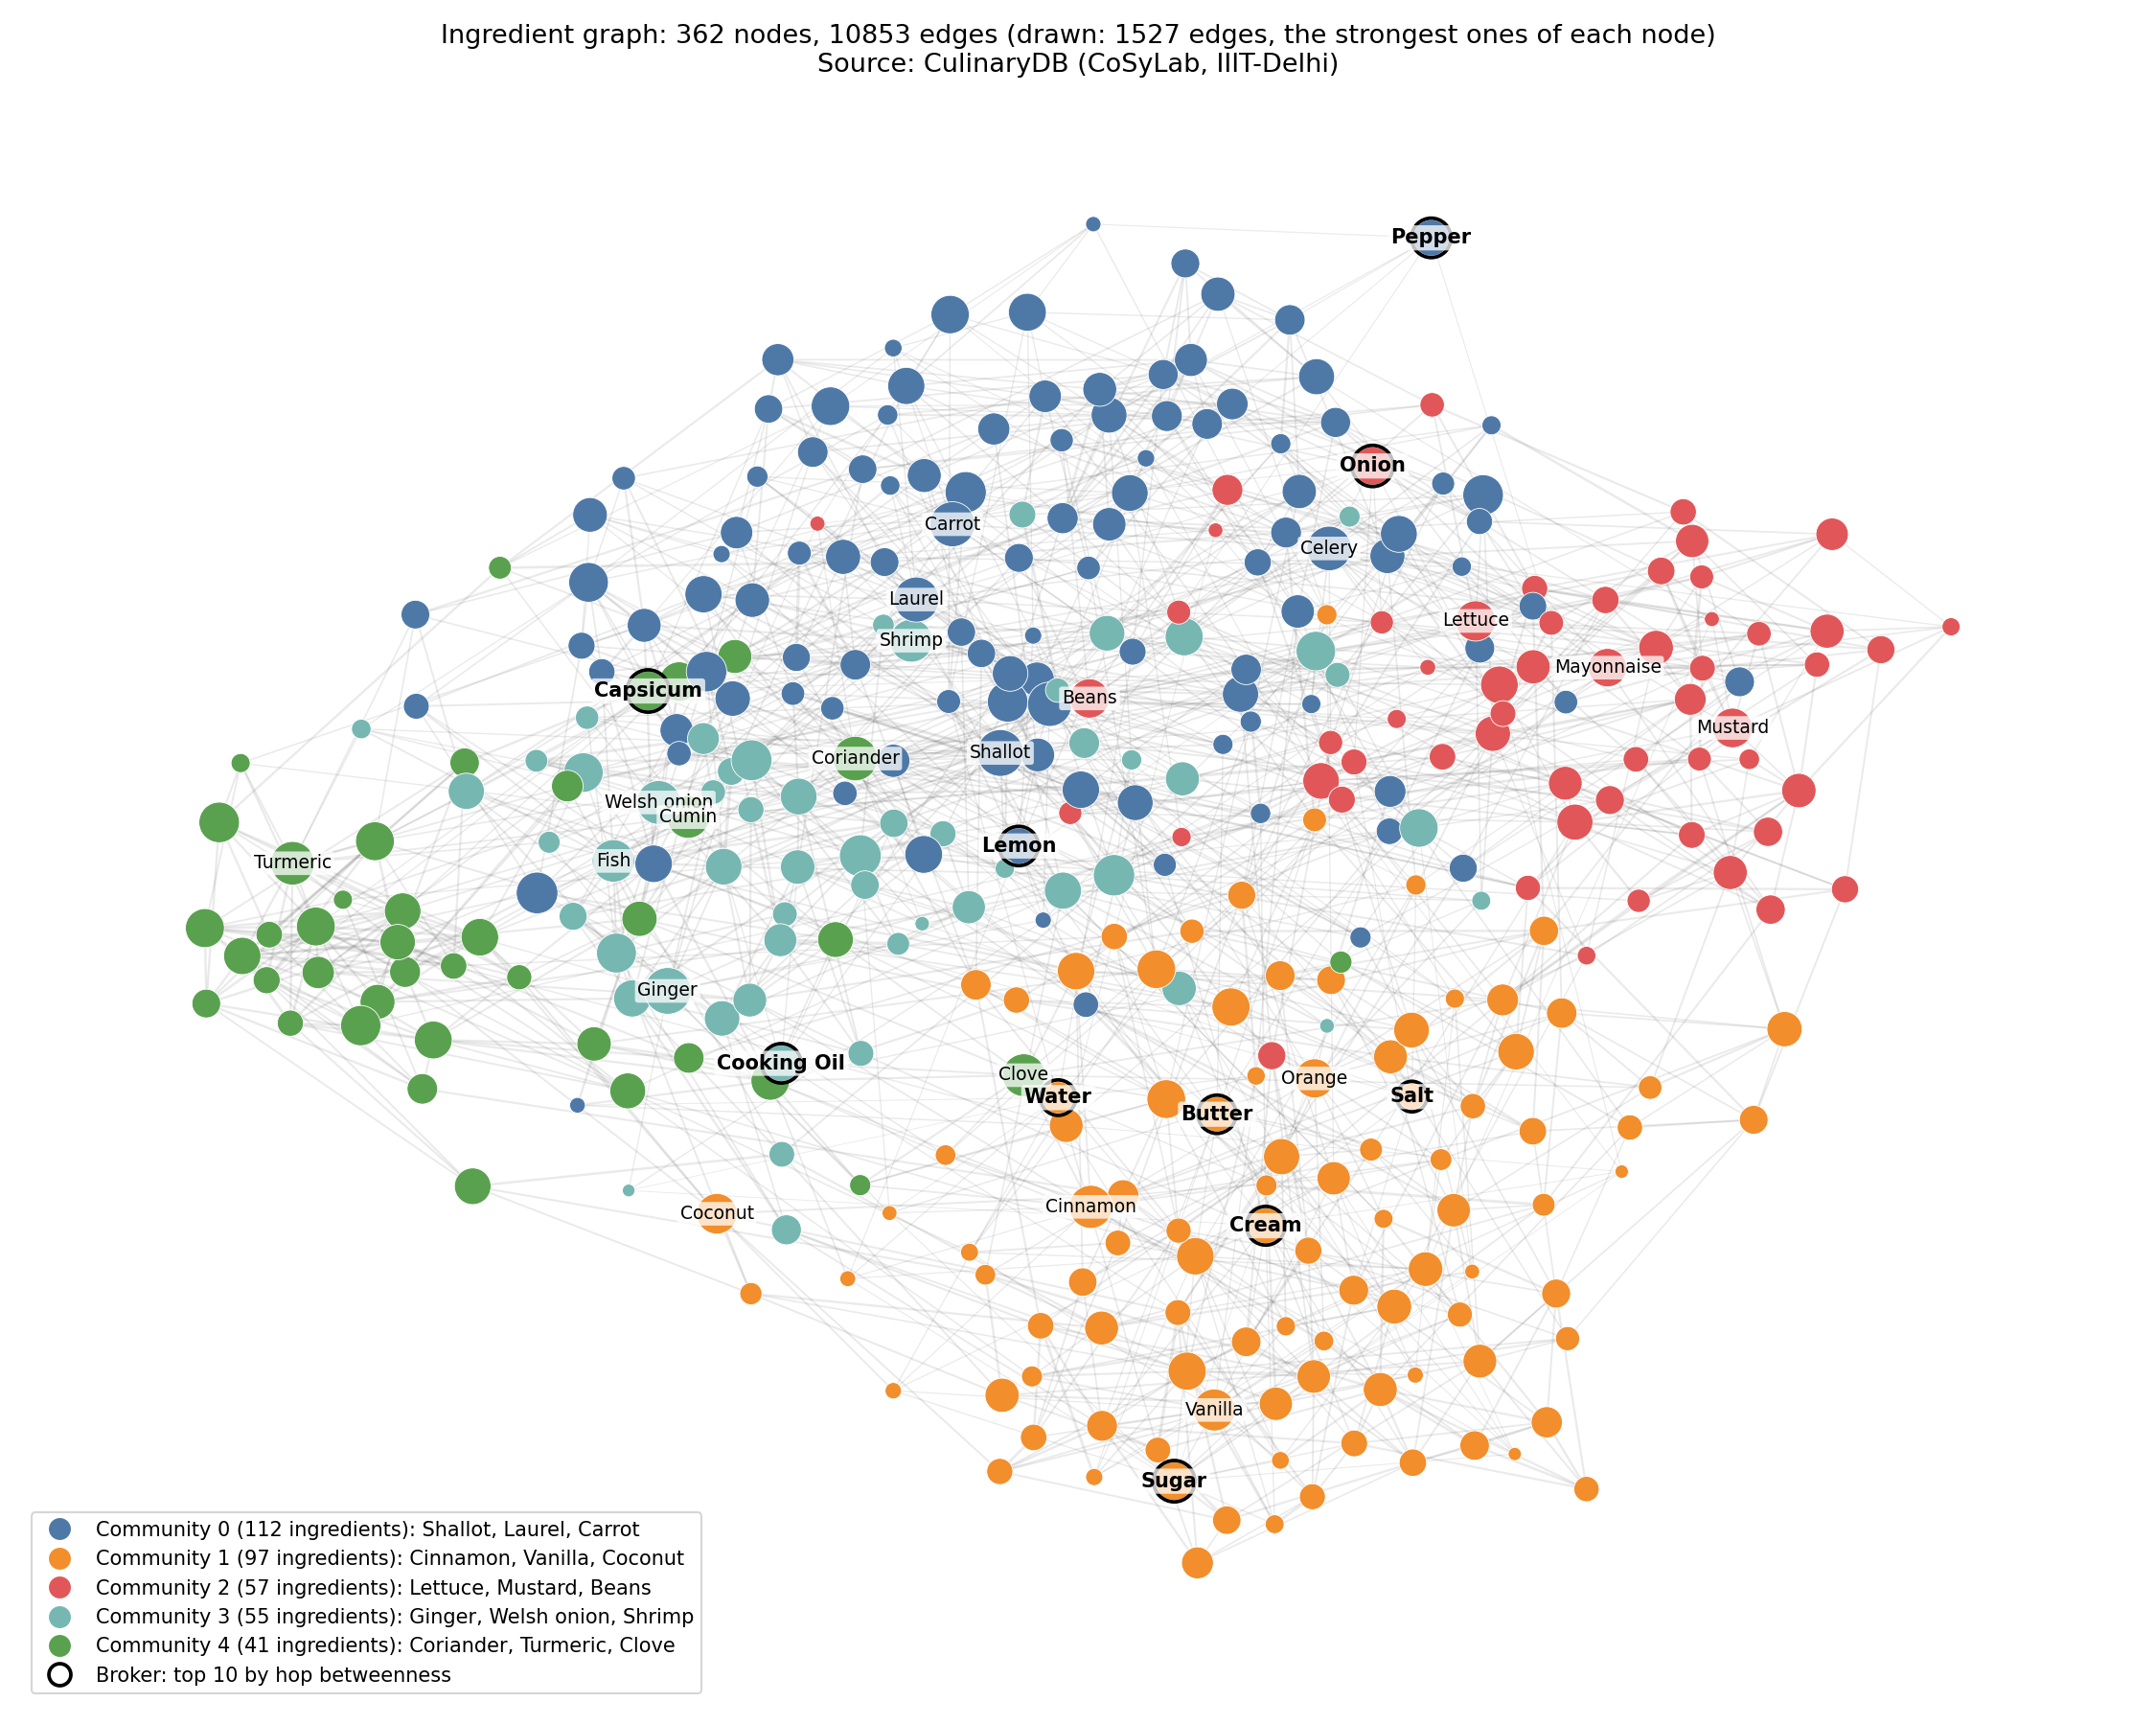
\includegraphics[width=\linewidth]{fig_ingredients.png}
%   \caption{TODO (English labels after the Friday fix).}
% \end{figure}


\subsection{Brokers: betweenness versus frequency}
% Owner: B
%% Owner: B. Hop betweenness leaders (Water, Salt, Butter, ...) track frequency
%% (Spearman 0.968): common ingredients are the path intermediaries. With 1/PMI
%% distances the leaders change (Couscous, Lasagna, Shallot, Coconut, Saffron;
%% Spearman 0.323), valid under that distance choice only. Inspect 2-3
%% ingredients in detail. The ingredient graph has no cut vertex or bridge.


\subsection{Countries and geography}
% Owner: B
We compare the country Louvain communities with UN regions in
Table~\ref{tab:regions}, the contingency table described in the analysis.
The majority share is the fraction of countries in a
community that belong to its most frequent region.

\begin{table}[h]
\centering
\small
\setlength{\tabcolsep}{4pt}
\begin{tabular}{@{}r r l c l@{}}
\toprule
Community & Size & Majority region & Share & Region counts \\
\midrule
0 & 49 & Europe & $31/49$ & Eu 31, Am 9, Af 4, As 3, Oc 2 \\
1 & 42 & Africa & $24/42$ & Af 24, Am 11, As 4, Eu 3 \\
2 & 32 & Asia & $21/32$ & As 21, Af 8, Eu 2, Am 1 \\
3 & 25 & Americas & $13/25$ & Am 13, Af 5, As 5, Oc 2 \\
4 & 9 & Asia & $9/9$ & As 9 \\
5 & 6 & Oceania & $5/6$ & Oc 5, Af 1 \\
6 & 3 & Oceania & $2/3$ & Oc 2, Af 1 \\
7 & 2 & Africa & $2/2$ & Af 2 \\
8 & 1 & Americas & $1/1$ & Am 1 \\
9 & 1 & Asia & $1/1$ & As 1 \\
10 & 1 & Oceania & $1/1$ & Oc 1 \\
\bottomrule
\end{tabular}
\caption{Country communities and UN regions. Shares are exact fractions.
Af = Africa, Am = Americas, As = Asia, Eu = Europe, Oc = Oceania;
omitted regions have no members. A majority region does not describe every
country in a mixed community.}
\label{tab:regions}
\end{table}

We find clear regional blocks: community $4$ contains $9$ Asian countries
out of $9$, and community $5$ contains $5$ countries in Oceania out of $6$.
The largest communities are mixed. Community $0$ contains $31$ European
countries and $9$ in the Americas, alongside other regions. Community $1$
contains $24$ African countries and $11$ in the Americas. We therefore do
not read the partition as a division into regions. Communities of sizes
$1$--$3$ partly reflect small dish profiles, which offer few ingredients
for comparing countries.

\paragraph{Shuffle test.}
Observed agreement is $0.643$, compared with a shuffled mean of $0.340$
and standard deviation $0.019$. The maximum over $1{,}000$ shuffles is
$0.404$, below the observed value (Figure~\ref{fig:shuffle}). No shuffle
reaches the observed agreement, giving $p=\frac{1}{1{,}001}\approx0.001$ with the
correction described in the analysis. Communities and UN regions are
therefore associated well beyond chance. This shows association, not cause,
and neighbouring countries are not independent.

\begin{figure}[h]
\centering
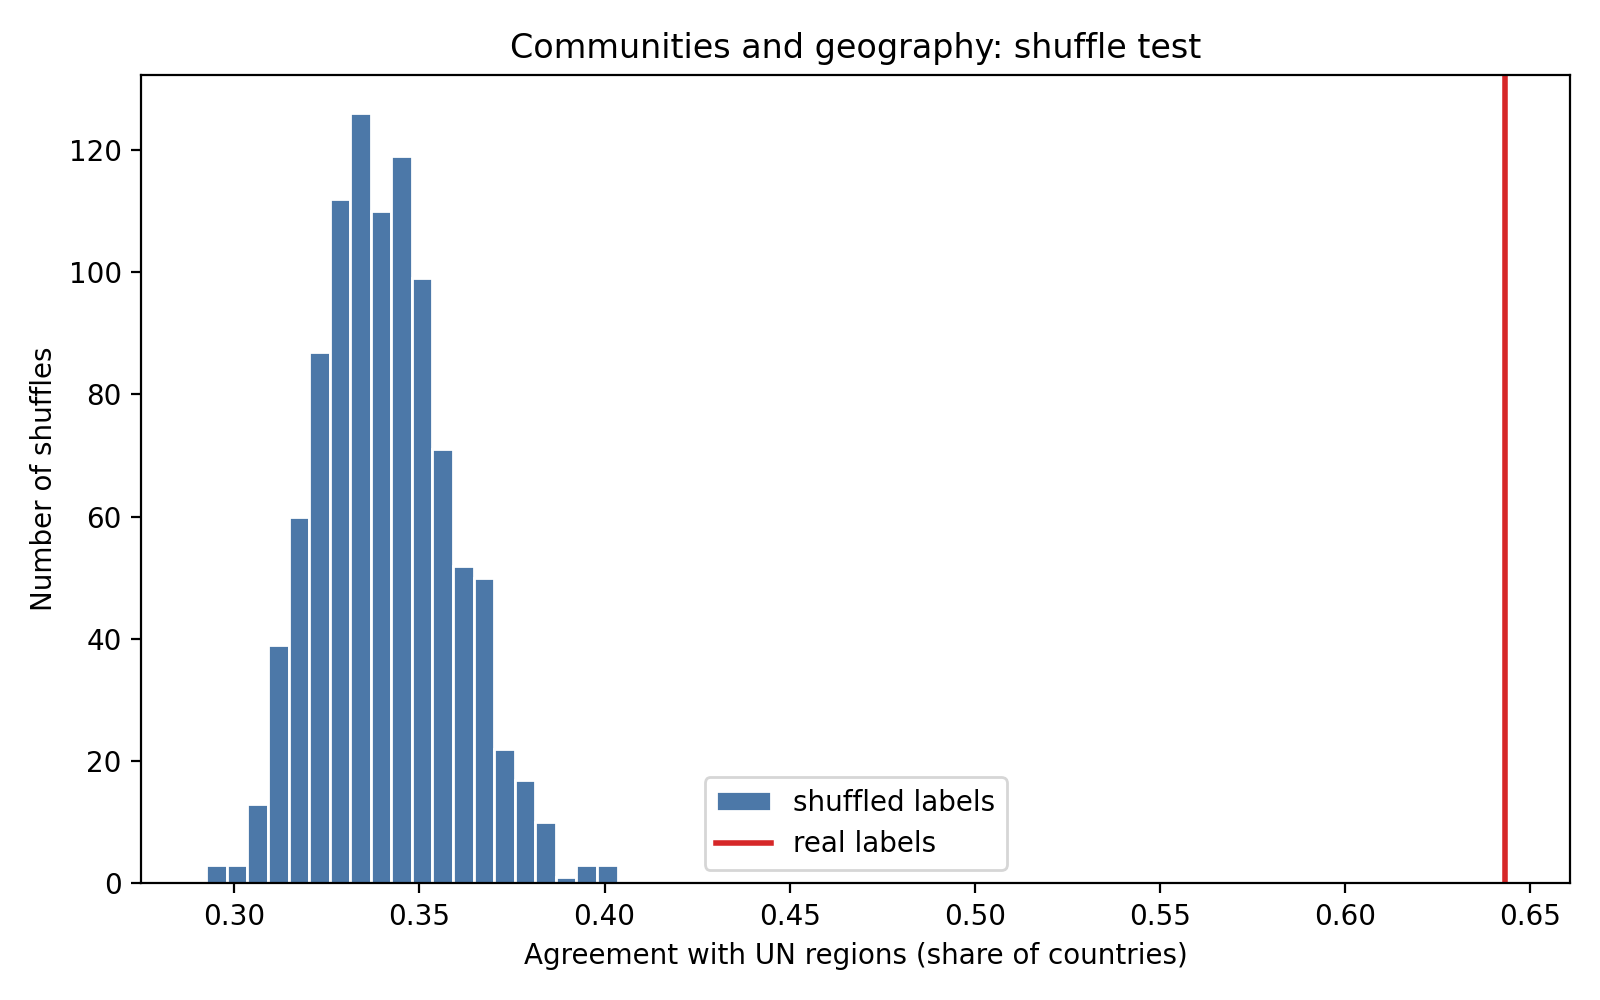
\includegraphics[width=0.75\linewidth]{shuffle_test.png}
\caption{Agreement with UN regions for the fixed Louvain communities:
1{,}000 shuffles of the region labels (bars) against the real labels (red line).}
\label{fig:shuffle}
\end{figure}

\paragraph{Connecting countries.}
Tonga, Fiji, Uganda, Mauritius and Tuvalu have the highest hop
betweenness. Betweenness follows degree less closely than for ingredients
($\rho=0.816$, against $0.973$), and the leaders are of two kinds. Fiji,
Uganda and Mauritius have many neighbours ($48$, $71$ and $66$), and most of
them lie in other communities ($62.5\%$, $76.1\%$ and $57.6\%$). These
outside neighbours span several regions: for Uganda, $26$ are in Africa,
$14$ in Asia, $8$ in the Americas and $6$ in Europe. These countries sit
between communities. Tonga and Tuvalu have only $9$ and $7$ neighbours.
Their betweenness comes from the bridges described below: every path from
Samoa passes through Tonga, and every path from Micronesia, Palau and
Seychelles passes through Tuvalu. Their rank therefore depends on small
profiles and on the threshold, like the cut points.

\paragraph{Cut points and small components.}
We find $5$ articulation points and $5$ bridges. Canada, Nicaragua and Samoa
each have a single neighbour (Belarus, Costa Rica and Tonga), so each hangs
on the rest of the graph by one bridge. Micronesia (Federated States of),
Palau and Seychelles form a small group attached only through the bridge
between Micronesia and Tuvalu. Outside the largest connected component,
Zambia and Zimbabwe form a component of two, and Grenada, Jordan and the
Marshall Islands are isolated. These countries have small dish profiles,
so a few ingredients decide whether they pass the Jaccard threshold of
$0.30$. We read these cut points as effects of the data and the threshold,
not as separations between cuisines.


\subsection{Sensitivity to thresholds}\label{sec:res-sensitivity}
% Owner: B
Table~\ref{tab:sensitivity} compares thresholds around our chosen settings.
We keep the country profile set to \texttt{all}, using the union of
ingredients from all dishes for each country.

\begin{table}[h]
\centering
\small
\setlength{\tabcolsep}{4pt}
\begin{tabular}{@{}l r r r r r@{}}
\toprule
Setting & Edges & Components & Largest & Communities & Modularity \\
\midrule
\multicolumn{6}{l}{Ingredients: minimum co-occurrence / PMI threshold} \\
\textbf{10 / 0.0} & 10{,}853 & 1 & 362 & 5 & 0.400 \\
10 / 0.5 & 7{,}745 & 1 & 362 & 5 & 0.423 \\
10 / 1.0 & 4{,}910 & 2 & 361 & 7 & 0.477 \\
20 / 0.0 & 7{,}873 & 3 & 360 & 8 & 0.414 \\
\midrule
\multicolumn{6}{l}{Countries: Jaccard threshold, profile \texttt{all}} \\
0.25 & 4{,}466 & 3 & 169 & 7 & 0.183 \\
\textbf{0.30} & 2{,}066 & 5 & 166 & 11 & 0.286 \\
0.35 & 835 & 17 & 153 & 23 & 0.437 \\
\bottomrule
\end{tabular}
\caption{Threshold comparisons, with our chosen settings in bold.
Largest gives the number of nodes in the largest connected component;
communities are found with Louvain. Modularity values describe different
graphs and must be read alongside their components.}
\label{tab:sensitivity}
\end{table}

At minimum co-occurrence $10$, increasing the PMI threshold from $0.0$ to
$0.5$ raises modularity from $0.400$ to $0.423$. The graph stays in one
connected component, so higher modularity here is not only a result of
splitting into components. Stricter settings also split the graph into
several components, which raises modularity on its own.

For countries, raising the Jaccard threshold from $0.25$ to $0.35$ raises
modularity from $0.183$ to $0.437$, but the number of components also grows
from $3$ to $17$. Part of that gain comes from the graph falling apart,
which is why we keep $0.30$.


% ============================================================================
\section{Conclusions}
% Owner: B
%% Owner: B drafts, both approve. Budget: 1 page.
\guidance{Summarize the main findings and note relevant limitations or possible future work.}
%% Direct answer to the central question. Limitations: sampled recipes, US/Italy
%% imbalance, small country profiles, seed dependence, one distance choice for
%% weighted betweenness. Future work in 2-3 lines.


\bibliographystyle{plain}
\bibliography{biblio}

\end{document}
